%%
%% This is file `sample-manuscript.tex',
%% generated with the docstrip utility.
%%
%% The original source files were:
%%
%% samples.dtx  (with options: `manuscript')
%% 
%% IMPORTANT NOTICE:
%% 
%% For the copyright see the source file.
%% 
%% Any modified versions of this file must be renamed
%% with new filenames distinct from sample-manuscript.tex.
%% 
%% For distribution of the original source see the terms
%% for copying and modification in the file samples.dtx.
%% 
%% This generated file may be distributed as long as the
%% original source files, as listed above, are part of the
%% same distribution. (The sources need not necessarily be
%% in the same archive or directory.)
%%
%% Commands for TeXCount
%TC:macro \cite [option:text,text]
%TC:macro \citep [option:text,text]
%TC:macro \citet [option:text,text]
%TC:envir table 0 1
%TC:envir table* 0 1
%TC:envir tabular [ignore] word
%TC:envir displaymath 0 word
%TC:envir math 0 word
%TC:envir comment 0 0
%%
%%
%% The first command in your LaTeX source must be the \documentclass command.
%%%% Small single column format, used for CIE, CSUR, DTRAP, JACM, JDIQ, JEA, JERIC, JETC, PACMCGIT, TAAS, TACCESS, TACO, TALG, TALLIP (formerly TALIP), TCPS, TDSCI, TEAC, TECS, TELO, THRI, TIIS, TIOT, TISSEC, TIST, TKDD, TMIS, TOCE, TOCHI, TOCL, TOCS, TOCT, TODAES, TODS, TOIS, TOIT, TOMACS, TOMM (formerly TOMCCAP), TOMPECS, TOMS, TOPC, TOPLAS, TOPS, TOS, TOSEM, TOSN, TQC, TRETS, TSAS, TSC, TSLP, TWEB.
% \documentclass[acmsmall]{acmart}

%%%% Large single column format, used for IMWUT, JOCCH, PACMPL, POMACS, TAP, PACMHCI
% \documentclass[acmlarge,screen]{acmart}

%%%% Large double column format, used for TOG
\documentclass[acmtog, authorversion]{acmart}
\usepackage[htt]{hyphenat}
\usepackage{graphicx}
\graphicspath{{images/}}
\usepackage[export]{adjustbox}
\usepackage{listings}
\usepackage{subfig}
\usepackage{pgfgantt}
\usepackage{tabularx}
\usepackage{longtable}
\usepackage{pgfplots}

\pgfplotsset{height=4.5cm,width=7.5cm,compat=1.18}

\setlength{\marginparwidth}{1.3cm}

\definecolor{prism_red}{rgb}{1.0, 0, 0}
\definecolor{prism_green}{rgb}{0, 0.6, 0}
\definecolor{prism_black}{rgb}{0, 0, 0}

\lstdefinelanguage{PRISM}{
    morekeywords={
     A, bool, clock, const, ctmc, C, double, dtmc, E, endinit, endinvariant, endmodule, endobservables, endrewards, endsystem, false, formula, filter, func, F, global, G, init, invariant, I, int, label, max, mdp, min, module, X, nondeterministic, observable, observables, of, Pmax, Pmin, P, pomdp, popta, probabilistic, prob, pta, rate, rewards, Rmax, Rmin, R, S, stochastic, system, true, U, W
    },
    otherkeywords={-, *, /, <, <=, >=, >, =, !=, !, &, |, <=>, =>, ?, :, [, ], (, ), ;, ..},
    sensitive=true,
    morecomment=[l]{//},
    morestring=[b]",
    basicstyle=\color{prism_red}\footnotesize\ttfamily,
    commentstyle=\color{prism_green},
    keywordstyle=\color{prism_black},
    breaklines=false
}

% \lstset{
%     language={PRISM},
%     basicstyle=\color{red}\tiny\ttfamily
%     commentstyle=\color{prism_green},
%     keywordstyle=\color{prism_black}
% }


%%%% Generic manuscript mode, required for submission
%%%% and peer review
%\documentclass[manuscript,screen,review]{acmart}
%% Fonts used in the template cannot be substituted; margin 
%% adjustments are not allowed.
%%
%% \BibTeX command to typeset BibTeX logo in the docs
\AtBeginDocument{%
  \providecommand\BibTeX{{%
    \normalfont B\kern-0.5em{\scshape i\kern-0.25em b}\kern-0.8em\TeX}}}

%% Rights management information.  This information is sent to you
%% when you complete the rights form.  These commands have SAMPLE
%% values in them; it is your responsibility as an author to replace
%% the commands and values with those provided to you when you
%% complete the rights form.

\setcopyright{acmcopyright}
\copyrightyear{2022}
\acmYear{2022}

%% These commands are for a PROCEEDINGS abstract or paper.
\acmConference[TScIT 37]{37$^{th}$ Twente Student Conference on IT}{July 8,
  2022}{Enschede, The Netherlands}
%
%  Uncomment \acmBooktitle if th title of the proceedings is different
%  from ``Proceedings of ...''!
%
%\acmBooktitle{Woodstock '18: ACM Symposium on Neural Gaze Detection,
% June 03--05, 2018, Woodstock, NY} 
%\acmPrice{15.00}
%\acmISBN{978-1-4503-XXXX-X/18/06}


%%
%% Submission ID.
%% Use this when submitting an article to a sponsored event. You'll
%% receive a unique submission ID from the organizers
%% of the event, and this ID should be used as the parameter to this command.
%%\acmSubmissionID{123-A56-BU3}

%%
%% For managing citations, it is recommended to use bibliography
%% files in BibTeX format.
%%
%% You can then either use BibTeX with the ACM-Reference-Format style,
%% or BibLaTeX with the acmnumeric or acmauthoryear sytles, that include
%% support for advanced citation of software artefact from the
%% biblatex-software package, also separately available on CTAN.
%%
%% Look at the sample-*-biblatex.tex files for templates showcasing
%% the biblatex styles.
%%

%%
%% The majority of ACM publications use numbered citations and
%% references.  The command \citestyle{authoryear} switches to the
%% "author year" style.
%%
%% If you are preparing content for an event
%% sponsored by ACM SIGGRAPH, you must use the "author year" style of
%% citations and references.
%% Uncommenting
%% the next command will enable that style.
%%\citestyle{acmauthoryear}
\setcitestyle{nosort}

%%
%% end of the preamble, start of the body of the document source.
\begin{document}

\renewcommand{\sectionautorefname}{Section}
\renewcommand{\subsectionautorefname}{Subsection}

%%
%% The "title" command has an optional parameter,
%% allowing the author to define a "short title" to be used in page headers.
\title[Analysis of Stochastic Behaviour in Sokoban]{Analysis of Stochastic Behaviour in Sokoban}

%%
%% The "author" command and its associated commands are used to define
%% the authors and their affiliations.
%% Of note is the shared affiliation of the first two authors, and the
%% "authornote" and "authornotemark" commands
%% used to denote shared contribution to the research.

\author{Bram Hagens}
\email{b.hagens@student.utwente.nl}
\affiliation{%
  \institution{University of Twente}
  \streetaddress{P.O. Box 217}
  \city{Enschede}
  \country{The Netherlands}
  \postcode{7500AE}
}



%%
%% By default, the full list of authors will be used in the page
%% headers. Often, this list is too long, and will overlap
%% other information printed in the page headers. This command allows
%% the author to define a more concise list
%% of authors' names for this purpose.
\renewcommand{\shortauthors}{Bram Hagens}

%%
%% The abstract is a short summary of the work to be presented in the
%% article.
\begin{abstract}
    Sokoban is a challenging puzzle game for both humans and computers. By modifying the game to include stochastic elements, Sokoban can be used to benchmark different probabilistic model checkers. Probabilistic model checkers are used to analyse systems that exhibit probabilistic behaviour. To improve the real-world performance of these tools, being able to benchmark them with a large variety of models is essential. This research introduces a novel tool that can generate probabilistic models from Sokoban levels in the PRISM and JANI formats. With tens of thousands of Sokoban levels readily available online, many models can easily be generated and can be used as a part of a more extensive benchmarking suite, which in turn can be used to determine and compare various performance aspects of probabilistic model checkers during probabilistic model checker competitions. Additionally, the paper includes preliminary benchmarks for the Storm, Modest and PRISM model checkers, as well as an analysis of their performance and the properties of the models. 
\end{abstract}

%%
%% The code below is generated by the tool at http://dl.acm.org/ccs.cfm
%% Please copy and paste the code instead of the example below.
%%Optional
%%
%%\begin{CCSXML}
%%<ccs2012>
%% <concept>
%%  <concept_id>10010520.10010553.10010562</concept_id>
%%  <concept_desc>Computer systems organization~Embedded systems</concept_desc>
%%  <concept_significance>500</concept_significance>
%% </concept>
%% <concept>
%%  <concept_id>10010520.10010575.10010755</concept_id>
%%  <concept_desc>Computer systems organization~Redundancy</concept_desc>
%%  <concept_significance>300</concept_significance>
%% </concept>
%% <concept>
%%  <concept_id>10010520.10010553.10010554</concept_id>
%%  <concept_desc>Computer systems organization~Robotics</concept_desc>
%%  <concept_significance>100</concept_significance>
%% </concept>
%% <concept>
%%  <concept_id>10003033.10003083.10003095</concept_id>
%%  <concept_desc>Networks~Network reliability</concept_desc>
%%  <concept_significance>100</concept_significance>
%% </concept>
%%</ccs2012>
%%\end{CCSXML}

%%\ccsdesc[500]{Computer systems organization~Embedded systems}
%%\ccsdesc[300]{Computer systems organization~Redundancy}
%%\ccsdesc{Computer systems organization~Robotics}
%%\ccsdesc[100]{Networks~Network reliability}

%%
%% Keywords. The author(s) should pick words that accurately describe
%% the work being presented. Separate the keywords with commas.
\keywords{Sokoban, probabilistic model checking, stochastic behaviour, model generation, JANI, PRISM, Modest, analysis.}

\settopmatter{printacmref=false}

%% A "teaser" image appears between the author and affiliation
%% information and the body of the document, and typically spans the
%% page.
\begin{teaserfigure}
  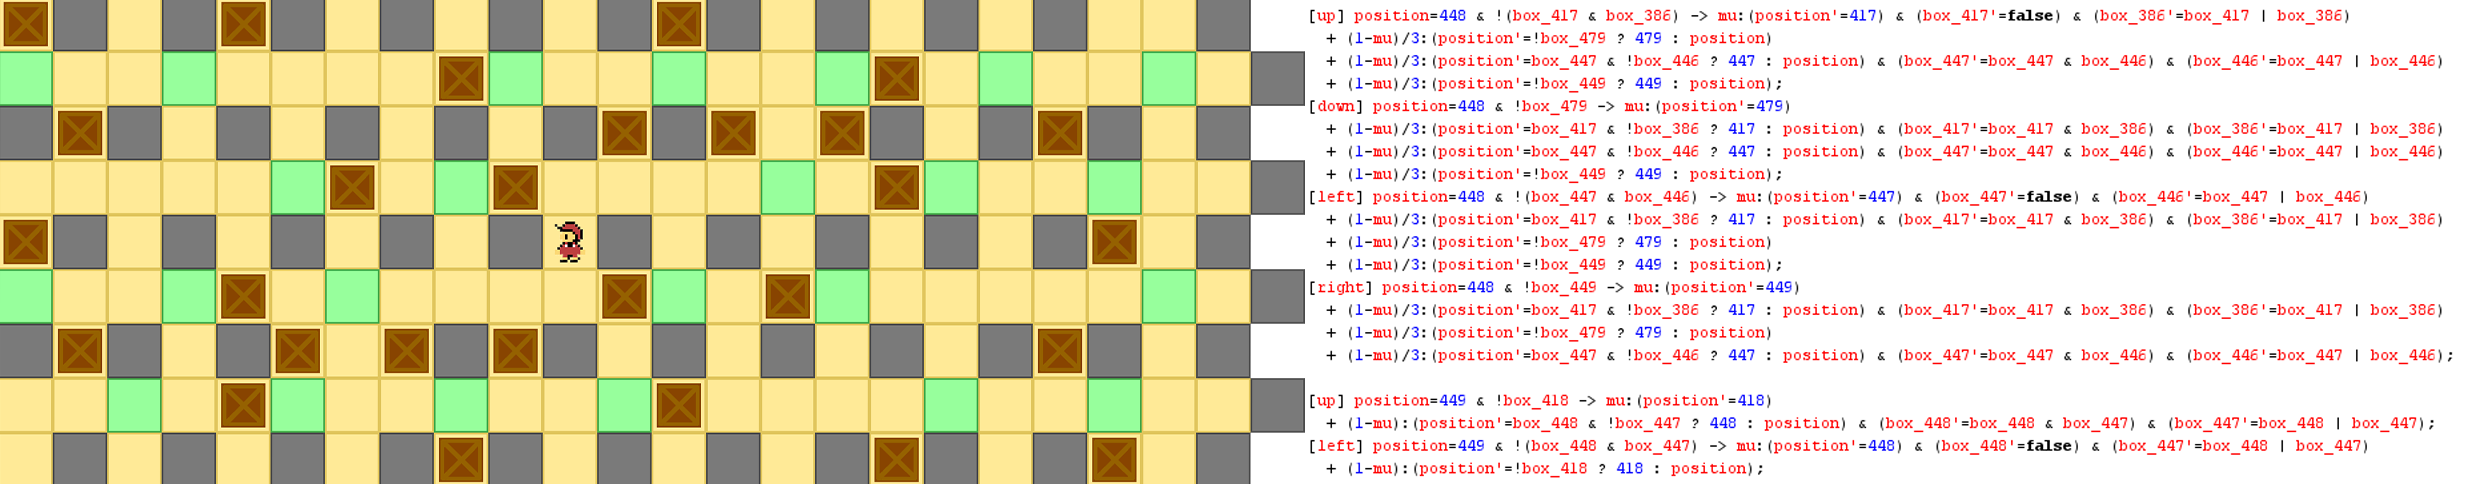
\includegraphics[width=\textwidth]{teaser}
  \caption{A Sokoban level next to a part of its probabilistic model representation.}
  \label{fig:teaser}
\end{teaserfigure}


%%
%% This command processes the author and affiliation and title
%% information and builds the first part of the formatted document.
\maketitle

\section{Introduction}
Systems that exhibit probabilistic behaviour exist everywhere: computer networks, security protocols, and traffic flows, among others. Using probabilistic model checking, a technique used to verify the correctness of a model of a stochastic system, one can compute bounds on the likelihood that a state will be reached. This can help prevent undesirable behaviour, such as a system crash or a deadlock. As these systems get more complex, it is important to use tools that can verify these models efficiently.

Sokoban is a puzzle game where a player pushes boxes into pre-defined locations. Solving Sokoban levels has been proven to be an NP-hard problem \cite{sokoban-np}. Introducing stochastic behaviour into this game will allow for the game to be used to benchmark probabilistic model checking tools. This is done by defining a probability that determines how often the model checker deviates from the shortest solution.

The goal of this research is to generate probabilistic models from Sokoban levels in various formats so that these models can be used as part of a more extensive test suite to benchmark existing probabilistic model checking tools in competitions such as QComp\footnote{\url{https://qcomp.org/}}.


\section{Background}
\subsection{Sokoban}
Sokoban is a single-player transport puzzle game where the player pushes boxes around into predetermined locations. A level is completed when all boxes are pushed into the correct spots. The player can move and push boxes in 4 directions: up, down, left and right, and is contained by walls surrounding the level. \autoref{fig:sokoban} shows an example of a simple Sokoban level. Not only is solving Sokoban puzzles NP-hard, but it is also proven to be PSPACE-complete\cite{pspace-complete}, making it significantly more difficult to solve than many other NP-hard problems. As a result, there exist many levels that state-of-the-art solvers cannot solve. 

\begin{figure}[h]
    \centering
    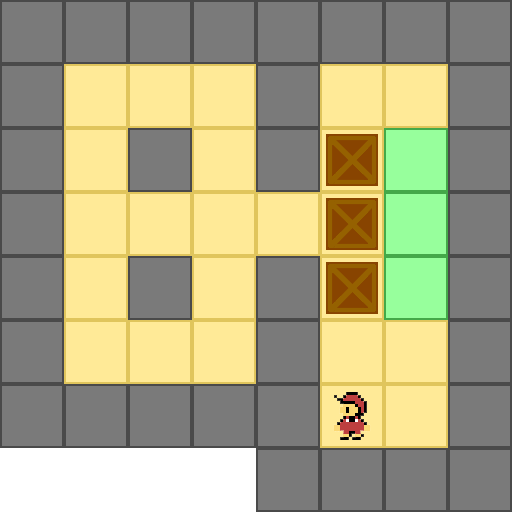
\includegraphics[width=5cm]{sokoban}
    \caption{An example Sokoban level. The gray tiles represent walls, the brown tiles represent boxes, and the green tiles are the targets.}
    \label{fig:sokoban}
\end{figure}

\subsection{Probabilistic model checking}
Model checking is a way of verifying the correctness of requirements of models. These models are often represented as finite-state machines. Using model checking tools, one can run queries on these state machines to verify the correctness of certain aspects of the model. A model of a Sokoban level would include the player and box positions, and the solution can be found by querying a state where all boxes are in the solved position. Probabilistic model checking is a similar technique that allows for verifying properties of models that exhibit stochastic behaviour. An example of such a model would be the model of a Sokoban level, but all inputs are randomly determined. One can now query the probability that the model ends up in an unsolvable state (e.g a box is pushed in a corner and can no longer move) or what the average length is to complete the level.

\subsection{Sok format}
.sok files\footnote{\url{http://www.sokobano.de/wiki/index.php?title=Sok_format}} are files that contain Sokoban levels. There are currently tens of thousands of user-created levels in this format freely available online. Apart from a few inconsistencies, the format is easy to parse and the large selection of levels makes it a good choice for this research. The contents of a .sok-file is depicted in \autoref{fig:sok}.

\lstset{basicstyle=\footnotesize\ttfamily,breaklines=true}

\begin{figure}[h]
    \subfloat[\centering ASCII representation of a .sok-file. '@' represents the player, '\$' represents a box, '.' represents a target location, and '\#' represents a wall.\label{fig:sok_ascii}]{\makebox[0.5\linewidth][c]{\lstinputlisting{code/level.sok}}}
    \hfill
    \subfloat[\centering Graphical representation of a .sok-file. The brown tiles represent boxes, the green tiles represent target locations, and the tiles blocks represent walls.]{\makebox[0.5\linewidth][c]{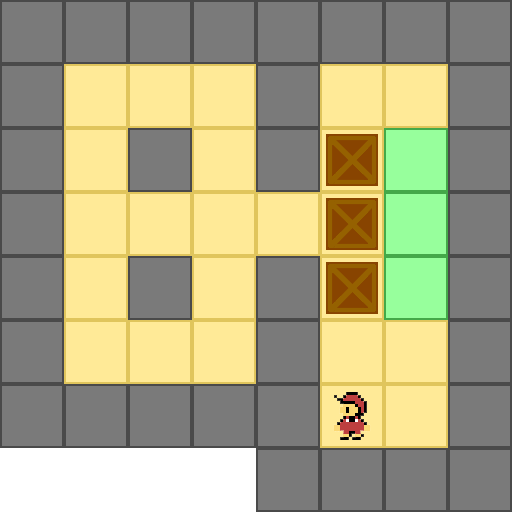
\includegraphics[width=3.5cm,valign=c]{sokoban.png}}}
    \caption{A .sok-file in both its ASCII and graphical representation.}
    \label{fig:sok}
\end{figure}


\section{Research questions}
\begin{enumerate}
    \item[\textbf{RQ1}.] To what extent do the stochastic additions influence the solutions generated by the model checker?
    \item[\textbf{RQ2}.] On average, which of the three model checkers, Storm, Modest, and PRISM, is the best suited for solving probabilistic Sokoban models?
\end{enumerate}

\section{Related work}
There exist many Sokoban solvers, such as Festival\footnote{\url{https://festival-solver.site/}} and Sokolution\footnote{\url{http://codeanalysis.fr/sokoban/}}. The goal of this research however is not to create a solver for (a stochastic version of) Sokoban, but to create a model that will be solved by a model checker.

A project similar to this research has been implemented that generates Sokoban models, which are then used to benchmark three different model checking tools: LTSmin, DiVinE and nuXmv\cite{comparing_sokoban}. It solely researched non-stochastic models, whereas this research only considers stochastic models and probabilistic model checking tools. While there was a comparison between a simple and more optimized model in that research, there was no attempt to find the optimal encoding of the player and box positions like there is in this research.

Similarly, another project focuses on generating models for various logic puzzles, including Sokoban, for LTSmin\cite{ltsmin-puzzles}. This research is different from the mentioned project for the same reasons as mentioned above.


\section{Modelling and Generation}

\subsection{Rules}
The models must abide by the following simple Sokoban rules: 
\begin{enumerate}
    \item A player can walk a single step at a time in any of the four directions (up, down, left, right) if there is not a box or a wall at the destination.
    \item A player can push a box in any of the four directions (up, down, left, right) if there is a box at the destination, and the tile behind the destination is not a box nor a wall.
\end{enumerate}

\subsection{Encoding}
The positions of the player and all boxes have to be encoded in a way that allows for a state to only be represented in one way, so that the state space will not be unnecessarily large. The position is stored as a simple integer bounded by the first and last reachable position on the board. For each reachable position, an additional flag is maintained that signals whether there is a box at that position. The encoding of the level depicted in \autoref{fig:sokoban_simple} is as follows:
\lstinputlisting[language=PRISM]{code/encoding.prism}
There are nine box flags, one for each reachable position. As the box is in position 12 initially, the flag corresponding to this position one is set to true. The player can move freely between the reachable tiles, given that there is no box or wall in the way, and their position is bounded by the first and last reachable tile index. According to the bounds, the player can reach invalid positions, such as a wall. The transitions of the model prevent this from happening.

\begin{figure}[h]
    \centering
    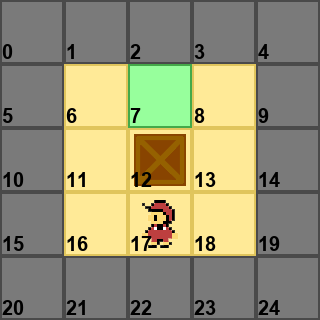
\includegraphics[width=4.5cm]{images/sokoban_simple.png}
    \caption{A simple Sokoban level with a position index on each tile.}
    \label{fig:sokoban_simple}
\end{figure}

\subsection{Non-deterministic transitions}
The probabilistic model is a Markov decision process (MDP). This type of model allows for both probabilistic and non-deterministic transitions. The moves in the model description are specified in such a way that they will be chosen non-deterministically. The moves can be in any direction, as long as the puzzle's layout allows for this. If the player is positioned at a tile $T$, they can walk to any adjacent tile $T'$, given that this tile is not a wall nor contains a box. If $T'$ does contain a box, the player will have to push the box forwards to the adjacent tile $T''$. This is only possible if $T''$ is not a wall nor contains a box. This means that for any combination of ($T$, $T'$), a walk transition exists, while a push transition between ($T$, $T'$) only exists if $T''$ is not a wall.

From position 12 in \autoref{fig:sokoban_simple}, only walk transitions exist, as the push condition cannot be satisfied. The transitions look as follows:
\lstinputlisting[language = PRISM]{code/walk_transitions.prism}
From all other reachable positions, the player can always push in one direction. Since the existence of a push transition into a direction also implies the existence of a walk transition into that same direction, the two moves are modelled as a single transition. This transition looks as follows from position 17:
\lstinputlisting[language=PRISM]{code/push_transition.prism}
The other two transitions, left and right, are again walk-only transitions. There is no down transition, as there is a wall at position 22.

Using these two types of transitions, a model checker can determine the shortest solution to this non-deterministic model.

\subsection{Probabilistic mistakes} 
Stochastic behaviour is added to the transitions, which forces the model checker to choose a suboptimal move with a predetermined probability. In this case, a suboptimal move is one that in most cases will increase the number of steps taken to solve the level. This behaviour is added by modifying the transitions so that with a probability of $\mu$, the player makes the optimal move. The remaining probability, $1 - \mu$, is divided into equal parts depending on the possible amount of alternative moves the player can make from that position. If the player cannot make the specified alternative move due to the current state of the board (for example because there are boxes in the way), the player does not move to prevent the model from deadlocking due to an invalid move.

The probabilistic up transition from position 12 in \autoref{fig:sokoban_simple} is modelled as follows:
\lstinputlisting[language=PRISM]{code/probabilistic_transition.prism}
From position 12, there are four possible walk moves: up, down, left, and right. The primary move, up in the example above, is chosen with a probability of $\mu$. The three alternative moves are chosen with a probability of $\frac{1 - \mu}{3}$. As only walk moves are permitted from this position, it is possible that a move cannot be executed because of a box being in the way. As mentioned above, the model must not deadlock due to invalid moves, thus the alternative moves are modelled using a ternary statement so that they are only executed if they are valid moves.

The concept remains the same if push moves are also permitted, however, due to the need to check and reassign more variables, these are more complex. The assignments for the walk/push move from position 12 to position 7 in \autoref{fig:sokoban_simple} are modelled as follows; for the sake of brevity, the guards and other irrelevant assignments are left out:
\lstinputlisting[language=PRISM]{code/probabilistic_push_transition.prism}

The probabilistic transitions have a significant consequence on the solvability of the levels. The model now forces the model checker to make a suboptimal move with the probability of $\mu$. While invalid moves will not be executed, it is now possible to make the level unsolvable by pushing a box into a position from which it can no longer be moved.

\subsection{Rewards}
\label{sec:rewards}
PRISM, Modest and Storm all support MDPs with transition rewards. This means that a certain cost can be attached to a transition, which can be used to calculate the total amount of moves taken to reach the required state. However, if the probability of reaching this state is less than 1, the rewards converge to infinity. Support for conditional reward properties for MDPs is missing in all three model checkers, meaning with the model described above, rewards cannot be used due to the fact that a mistake could make the level unsolvable. However, to still be able to calculate the expected amount of moves required to solve the level, the generation tool can also output models where a mistake can only be a walk move, not a push move. This means a level will never be unsolvable, as a walk move can always be undone; thus, the rewards work as expected.

\subsection{Generation}
The model generation tool generates probabilistic models as described above from Sokoban levels supplied by the user as .sok files. The generated models are described by the PRISM language and the JANI specification so that a wide range of probabilistic model checkers can be targeted. The generated models contain an undefined constant, $\mu$, that defines the probability that the player makes the best move. A high-level overview of the workings of the tool is as follows:
\begin{enumerate}
    \item Parse a .sok file into an intermediate representation that better suits the generation process.
    \item Run a depth-first search starting from the player's position to find all reachable tiles.
    \item Generate the variables used to encode the player and box positions.
    \item Iterate over all possible moves for each reachable tile and generate the transitions between the states.
\end{enumerate}


\section{Method}
The research consists of two parts: (a) generating probabilistic models from existing Sokoban levels and a set of probabilities, and (b) experimenting with the generated models. 

For part a., stochastic behaviour has to be introduced to the non-stochastic game Sokoban. This is done by defining the following probabilities:
\begin{enumerate}
    \item The probability that decides if the player's move is respected, or if a different move is selected. Additionally, probabilities for each movement direction are defined.
    \item The probability that a box moves when not pushed by a player. Additionally, probabilities for each movement direction are defined.
\end{enumerate}

The probabilistic models are derived from .sok files, and the models are described by the PRISM language\cite{prism} and the JANI specification\cite{jani}, so that a wide range of probabilistic model checkers can be targetted. The goal is to create a tool that automates this process: using a .sok file and a set of probabilities as input, it should be able to output a probabilistic model in either the PRISM language, JANI, or both.

Additionally, the position of the player and the boxes are represented in multiple ways. Depending on how these values are encoded, the performance of the model checkers may differ.

The generated models abide by the following transition rules:
\begin{enumerate}
    \item The player can walk in any of the four directions (up, down, left, right) if:
    \begin{enumerate}
        \item there is not a box or wall at the destination. This action updates the player's position to the destination.
        \item there is a box at the respective destination and the tile behind the destination is not a wall nor box. This action moves the box one tile backwards, and updates the player's position to the destination.
    \end{enumerate}
\end{enumerate}

These transition rules do mean that it is possible to end up in unsolvable states: a player is able to position boxes in such a way that they can no longer push them, or they can lock themselves into an area of the level without being able to escape. However, with the stochastic additions it is possible that these situations resolve themselves eventually, whereas for the non-stochastic version of Sokoban one of those scenarios would most certainly require the player to reset from the start.


Part b. involves experimenting with the generated models using existing probabilistic modelling tools. The tests will be conducted in virtual machines with identical specifications running an identical operating system. This creates a consistent playing field for the model checkers so that the run time performance can be measured fairly. Depending on the duration of the tests, they will be run multiple times to reduce inconsistencies caused due to measurement errors. A test is deemed completed once the target state is reached.


% Part b. involves experimenting with the generated models using existing model checkers. Using these existing checkers, various stochastic properties can be verified about the models, such as:
% \begin{itemize}
%     \item The probability that a legal, unsolvable state is reached.
%     \item The probability that the target state is reached.
%     \item The probability that the target state is reached in less steps than the non-stochastic minimum solution.
% \end{itemize} 

% Additionally, during the generation phase, models can be generated in different ways. This may or may not improve performance for one or more checkers. By adding more constraints on what is and what is not considered a valid move, the state space can be reduced significantly. This can be done by disallowing moves that cause boxes to be stuck in corners or that moves that otherwise create an unsolvable state. These models will be referred to as the optimized models.

% Furthermore, 

% This yields the following research questions:
% \begin{enumerate}
%     \item What properties are interesting?
%     \todo[inline]{Poorly formulated RQ}
%     \item What is the effect of the optimization of the model on the run time and state space of the model checker?
% \end{enumerate}
% \todo[inline]{Something about model type?}
% \todo[inline]{Something about player/box position encoding?}

% \section{Method}
% A Sokoban level, in the sok format as depicted in \autoref{fig:sok_ascii}, is used as an input for a program. The program also requires a set of probabilities to be defined for the stochastic behaviour described in \autoref{sec:problem_statement}. It will output two models: one described in the PRISM language and one according to the JANI specification.

% For the regular models, the following transition rules are specified:
% \begin{itemize}
%     \item The player can walk in any of the four directions (up, down, left, right) if:
%     \begin{itemize}
%         \item there is not a box or wall at the destination. This action updates the player's position to the destination.
%         \item there is a box at the respective destination and the tile behind the destination is not a wall nor box. This action moves the box one tile backwards, and updates the player's position to the destination.
%     \end{itemize}
% \end{itemize}

% Additionally, for the optimized models the following rules are added:
% \begin{itemize}
%     \item A player may not push a box into a corner of the walls, unless this is required to reach the target state.
%     \item A player may not box themselves in by placing boxes in a way that they can no longer reach the target state.
% \end{itemize}
% Both these rules exist as there is no way to recover from these states. It is impossible to retrieve a box when it is placed in a corner, as a box can only be pushed from behind and the player is unable to phase through walls. When the level has multiple levels, in some cases it is possible that the player boxes themselves in by placing the boxes in such a way that their exit is cut off and they can no longer move the blocking boxes out of the way. By adding these two rules, it is possible that the state space will be reduced as there will be less solutions that end in an unsolvable state.

% The JANI model is run in mcsta, part of the Modest Toolset\footnote{\url{https://www.modestchecker.net/}}. The PRISM model is ran in PRISM. The tests will be conducted in virtual machines running Ubuntu 64-bit 20.04.4 LTS. Both machines have access to 1 CPU core, 20GB of storage space and 8 GB of RAM. This creates a consistent playing field for the model checkers so that run time performance can be measured fairly. Tests will be run 5 times and the run time will be averaged to smooth out any inconsistencies due to measurement errors. A test will be completed when the target state is reached, with a maximum time of 5 minutes before the test is deemed a failure.


\begin{table*}[ht]
\begin{tabularx}{\textwidth}{XX|XX|XX|}
\cline{3-6}
                                       &             & \multicolumn{2}{l|}{All}                                                   & \multicolumn{2}{l|}{Shared}                                                \\ \hline
\multicolumn{1}{|l|}{Checker (engine)} & Num. solved & \multicolumn{1}{l|}{Avg. runtime solved (s)} & Avg. peak memory use solved (MB) & \multicolumn{1}{l|}{Avg. runtime solved (s)} & Avg. peak memory use solved (MB) \\ \hline
\multicolumn{1}{|l|}{PRISM (hybrid)}   & 127         & \multicolumn{1}{l|}{27}                      & 296                         & \multicolumn{1}{l|}{16}                      & 260                         \\ \hline
\multicolumn{1}{|l|}{Storm (hybrid)}   & 130         & \multicolumn{1}{l|}{35}                      & 2792                        & \multicolumn{1}{l|}{18}                      & 2831                        \\ \hline
\multicolumn{1}{|l|}{Modest (mcsta)}   & 121         & \multicolumn{1}{l|}{26}                      & 267                         & \multicolumn{1}{l|}{23}                      & 255                         \\ \hline
\end{tabularx}
\caption{Result of the benchmarks on the Microban level set for $\mu=0.3$. The \textit{All} column takes all solved levels into account, while the \textit{Shared} column only counts the levels that are solved by all model checkers.}
\label{tab:benchmark_mu_0.3}
\end{table*}

\begin{table*}[ht]
\begin{tabularx}{\textwidth}{XX|XX|XX|}
\cline{3-6}
                                       &             & \multicolumn{2}{l|}{All}                                                   & \multicolumn{2}{l|}{Shared}                                                \\ \hline
\multicolumn{1}{|l|}{Checker (engine)} & Num. solved & \multicolumn{1}{l|}{Avg. runtime solved (s)} & Avg. peak memory use solved (MB) & \multicolumn{1}{l|}{Avg. runtime solved (s)} & Avg. peak memory use solved (MB) \\ \hline
\multicolumn{1}{|l|}{PRISM (hybrid)}   & 128         & \multicolumn{1}{l|}{15}                      & 299                         & \multicolumn{1}{l|}{13}                      & 278                         \\ \hline
\multicolumn{1}{|l|}{Storm (hybrid)}   & 138         & \multicolumn{1}{l|}{37}                      & 2811                        & \multicolumn{1}{l|}{26}                      & 2853                        \\ \hline
\multicolumn{1}{|l|}{Modest (mcsta)}   & 131         & \multicolumn{1}{l|}{22}                      & 518                         & \multicolumn{1}{l|}{22}                      & 524                         \\ \hline
\end{tabularx}
\caption{Result of the benchmarks on the Microban level set for $\mu=0.9$. The \textit{All} column takes all solved levels into account, while the \textit{Shared} column only counts the levels that are solved by all model checkers.}
\label{tab:benchmark_mu_0.9}
\end{table*}

\begin{figure}[h]
    \centering
    \begin{tikzpicture}
    \begin{axis}[
        title={Pmax=? [F "goal\_reached"]},
        xlabel = $\mu$,
        ylabel = Max probability,
        ytick = {0, 0.25, 0.5, 0.75, 1}
    ]
    \addplot table [only marks, x=mu, y=probability, col sep=comma] {data/goal_state_reached.csv};
    \end{axis}
    \end{tikzpicture}
    \caption{Average maximum probability of the goal state being reached based on the value of $\mu$ for the Microban level set (n=92).}
    \label{fig:chart_goal_reached}
\end{figure}

\begin{figure}[h]
    \centering
    \begin{tikzpicture}
    \begin{axis}[
        title={Pmax=? [F<=t "goal\_reached"]},
        ymode=log,
        xlabel = $\mu$,
        ylabel = Max probability,
        ytick={1, 0.001, 0.000001, 0.000000001, 0.000000000001}
    ]
    \addplot table [only marks, x=mu, y=probability, col sep=comma] {data/optimal_solution.csv};
    \end{axis}
    \end{tikzpicture}
    \caption{Average maximum probability of the goal state being reached in $t$ moves based on the value of $\mu$ for the Microban level set, where $t$ is the minimum amount of moves required to solve the level (n=103).}
    \label{fig:chart_optimal_solution}
\end{figure}

\begin{figure}[h]
    \centering
    \begin{tikzpicture}
    \begin{axis}[
        title={Rmin=? [F "goal\_reached"]},
        xlabel = $\mu$,
        ylabel style={align=center}, ylabel= Difference from minimum\\number of moves (\%),
        ytick = {0, 500, 1000, 1500, 2000}
    ]
    \addplot table [only marks, x=mu, y=percentual_diff, col sep=comma] {data/expected_moves.csv};
    \end{axis}
    \end{tikzpicture}
    \caption{Average expected number of moves required to solve the level based on the value of $\mu$ for the Microban level set, expressed relative to the number of moves to reach the optimal solution (n=84).}
    \label{fig:chart_expected_moves}
\end{figure}

\section{Results}

The results for RQ1 are presented in \autoref{fig:chart_goal_reached}, \autoref{fig:chart_optimal_solution}, and \autoref{fig:chart_expected_moves}. The results for RQ2 can be found in \autoref{tab:benchmark_mu_0.3} and \autoref{tab:benchmark_mu_0.9}. All unsolved models were due to the time constraints imposed on the experiment, as none of the model checkers came close to the memory limit of 8 GB.



\section{Discussion}

\subsection{Analysis of stochastic additions to Sokoban}
\label{sec:property_analysis}
The stochastic additions greatly influence the generated solutions by the model checkers. As evident from \autoref{fig:chart_goal_reached}, making mistakes will significantly decrease the probability of being able to complete the level. This is expected, as a single push in the wrong direction will often cause a level to become unsolvable. The probabilities for $\mu<0.2$ have not been calculated due to the high level of iterations required to calculate the probability of solving the level with small $\mu$-values.

\autoref{fig:chart_optimal_solution} shows that the player often cannot recover and find an optimal solution if a mistake was made. However, in very few cases, there are two or more optimal solutions and a mistake will put the player on the path from one optimal solution to another optimal solution. 

As expected, a strong correlation exists between $\mu$ and the expected number of moves to solve a level, as shown in \autoref{fig:chart_expected_moves}. The fewer mistakes the player makes, the fewer moves are required to solve the level. The irregularities in this figure can be attributed to the smaller sample size for this experiment. Increasing the sample size should smoothen out the curve in the plot. The generated models are modified for this specific property, as explained in \autoref{sec:rewards}. This means that in most cases, a mistake is simply corrected by undoing the last move and carrying on with the optimal solution. If conditional properties with rewards were supported, the expected number of moves would likely be higher, as in most cases a wrong push move will need multiple moves to correct. 

\subsection{Benchmarks of PRISM, Storm, and Modest}
For both $\mu=0.3$ and $\mu=0.9$, Storm using the hybrid engine was able to solve the most Sokoban levels out of the test set within the 5-minute time limit. However, this comes at the cost of runtime performance and memory usage, as it performed the worst in these classes for both the \textit{All} and \textit{Shared} categories.

The most memory-efficient model checker for $\mu=0.3$ is Modest using the mcsta engine in both the \textit{All} and \textit{Shared} categories. For $\mu=0.9$, PRISM is the most memory-efficient in both categories. None of the model checkers exceeded the 8 GB memory limit before the timeout of 5 minutes was reached.

In general, PRISM with the hybrid engine is the fastest model checker. For the \textit{All} category for $\mu=0.3$, Modest was able to beat the average runtime by one second.

This proves that Storm is the most effective probabilistic model checker for this test set according to these measurements, as it was able to solve the greatest amount of models within the time and memory constraints out of the three model checkers. All model checkers were run with their default configuration, meaning there may have been configurations available that would yield more optimal results. This is outside the scope of this research.

As evident by the results analysed in \autoref{sec:property_analysis}, a lower value of $\mu$ reduces the probability of a valid solution being found. This can also be seen by comparing \autoref{tab:benchmark_mu_0.3} and \autoref{tab:benchmark_mu_0.9}: On average, levels were solved quicker for $\mu=0.9$ than for $\mu=0.3$.

\section{Conclusion}
Out of the three model checkers tested, Storm is the most capable of solving the probabilistic Sokoban levels. However, this comes at the cost of increased memory usage and a higher average time to solve levels. None of the model checkers ran out of memory within the time constraints. However, Storm used more than five times the amount of memory than the other tested model checkers.

The stochastic additions to the Sokoban game greatly influence the solutions generated by the model checkers. On average, the parameter that controls how often a player makes a mistake, $\mu$, determines how difficult the model will be to solve for the model checker. The higher the probability of making a mistake, the longer it takes for the model checker to solve certain properties, such as finding the maximum probability of completing the level.

\section{Future work}
The generated can be optimised further by reducing the bounds of the player position. Currently, it is bound between the lowest and highest reachable position index, but it is possible that many of these values in between the bounds are walls and thus not valid player positions. A solution to this would be to map all the positions on the board to a unique integer in the range $[0..n)$, with $n$ being the number of reachable tiles on the level. That way, all invalid positions are no longer considered, and the player's position will be bounded between $0$ and $n-1$.

In some cases, transitions are generated with guards that can never be satisfied. This can be a walk move towards an immovable box, or a push move where it is impossible for the player and box to be in those specific positions. Additionally, immovable boxes on a goal position are still considered when determining if a level is solved or not; these can also be optimised away. 

As described in \autoref{sec:rewards}, the model is modified to determine the expected number of moves. This influences the resulting amount of moves and thus is not optimal. This can be solved by using conditional reward properties to find the expected amount of moves for all solutions that reach the goal state. Baier et al. give an intricate solution for this \cite{Baier2017}. However, this method is not implemented in PRISM, Storm or Modest. An extension for PRISM is available that supports conditional properties, but rewards are not supported \cite{Mrcker2017}.

%%
%% The next two lines define the bibliography style to be used, and
%% the bibliography file.
\bibliographystyle{ACM-Reference-Format}
\bibliography{bibliography}

\end{document}
\endinput
